%
% Draft  document qgwrinkle.tex
% Notes on genetic analysis of ab32 and ab20 skin and wool data
%
 
\documentclass[titlepage]{article}  % Latex2e
\usepackage{graphicx,lscape,subfigure}
\usepackage{bm,longtable}
\usepackage{textcomp}
 

\title{ Quantitative genetics of skin wrinkle in sheep}
\author{Neville Jackson and Jim Watts }
\date{27 Jul 2018} 

 
\begin{document} 
 
\maketitle      
\tableofcontents


\clearpage
\section{Introduction} 
 The purpose of this investigation is to take a close look at the quantitative genetics of wrinkle score in Merino sheep.  Recent advances in our understanding of wrinkle formation (Watts personal communication) suggest that there may be maternal effects, with temperature regulation in the mother affecting skin development in the foetus. A close look at modes of inheritance  of wrinkle, other than by simple additive genes, is also warranted. There is a summary of what is known about additive genetics of wrinkle score in Jackson and Watts(2017)~\cite{jack:17a}.

\section{ Sheep population studied}
Data from CSIRO sheep breeding experiments (AB1, AB20, and AB32 in CSIRO jargon) is utilised.  These are all medium and fine wool Merino sheep. The AB1 experiment is documented in Turner etal(1968)~\cite{turn:68}, the AB20 experiment in Watson, Jackson, and Whiteley(1977)~\cite{wats:77}, and the AB32 experiment in Jackson(2017)~\cite{jack:17}.


Pedigree information was available on all sheep.

\section{Traits measured}
 Wrinkle scores on all of the above flocks were made according to the photographic standards of Turner etal(1953)~\cite{turn:53}. These photo standards are reproduced here (Figures~\ref{fig:wrneck} , ~\ref{fig:wrbody} and ~\ref{fig:wrbreech}). 
%\documentclass{article}
%\usepackage{graphicx,subfigure}
%\begin{document}

\begin{figure}[!h]
  \centering
   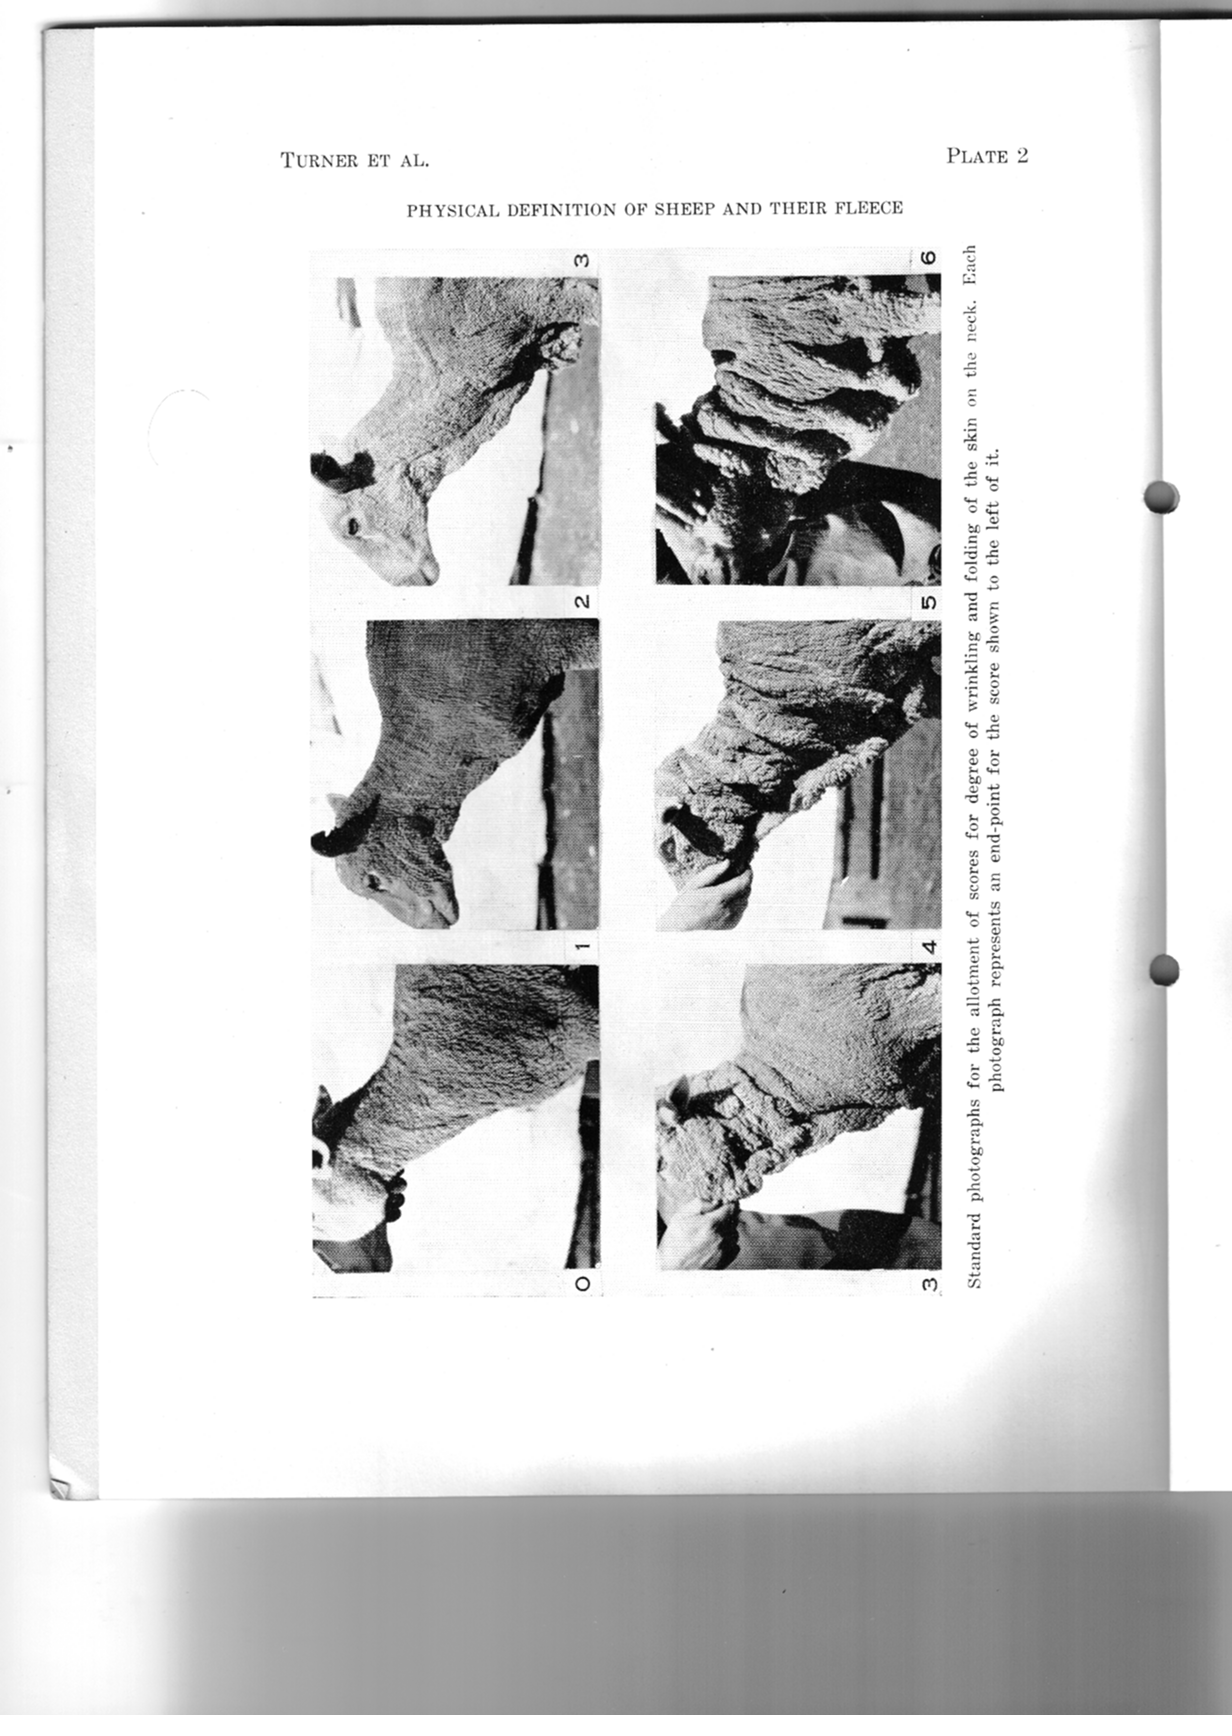
\includegraphics[width=0.9\textwidth]{wrneck.png}
  \caption{Photographic standards for sheep neck wrinkle scores from Turner etal(1953)~\cite{turn:53}}
  \label{fig:wrneck}
\end{figure}

%\end{document}


%\documentclass{article}
%\usepackage{graphicx,subfigure}
%\begin{document}

\begin{figure}[!h]
  \centering
   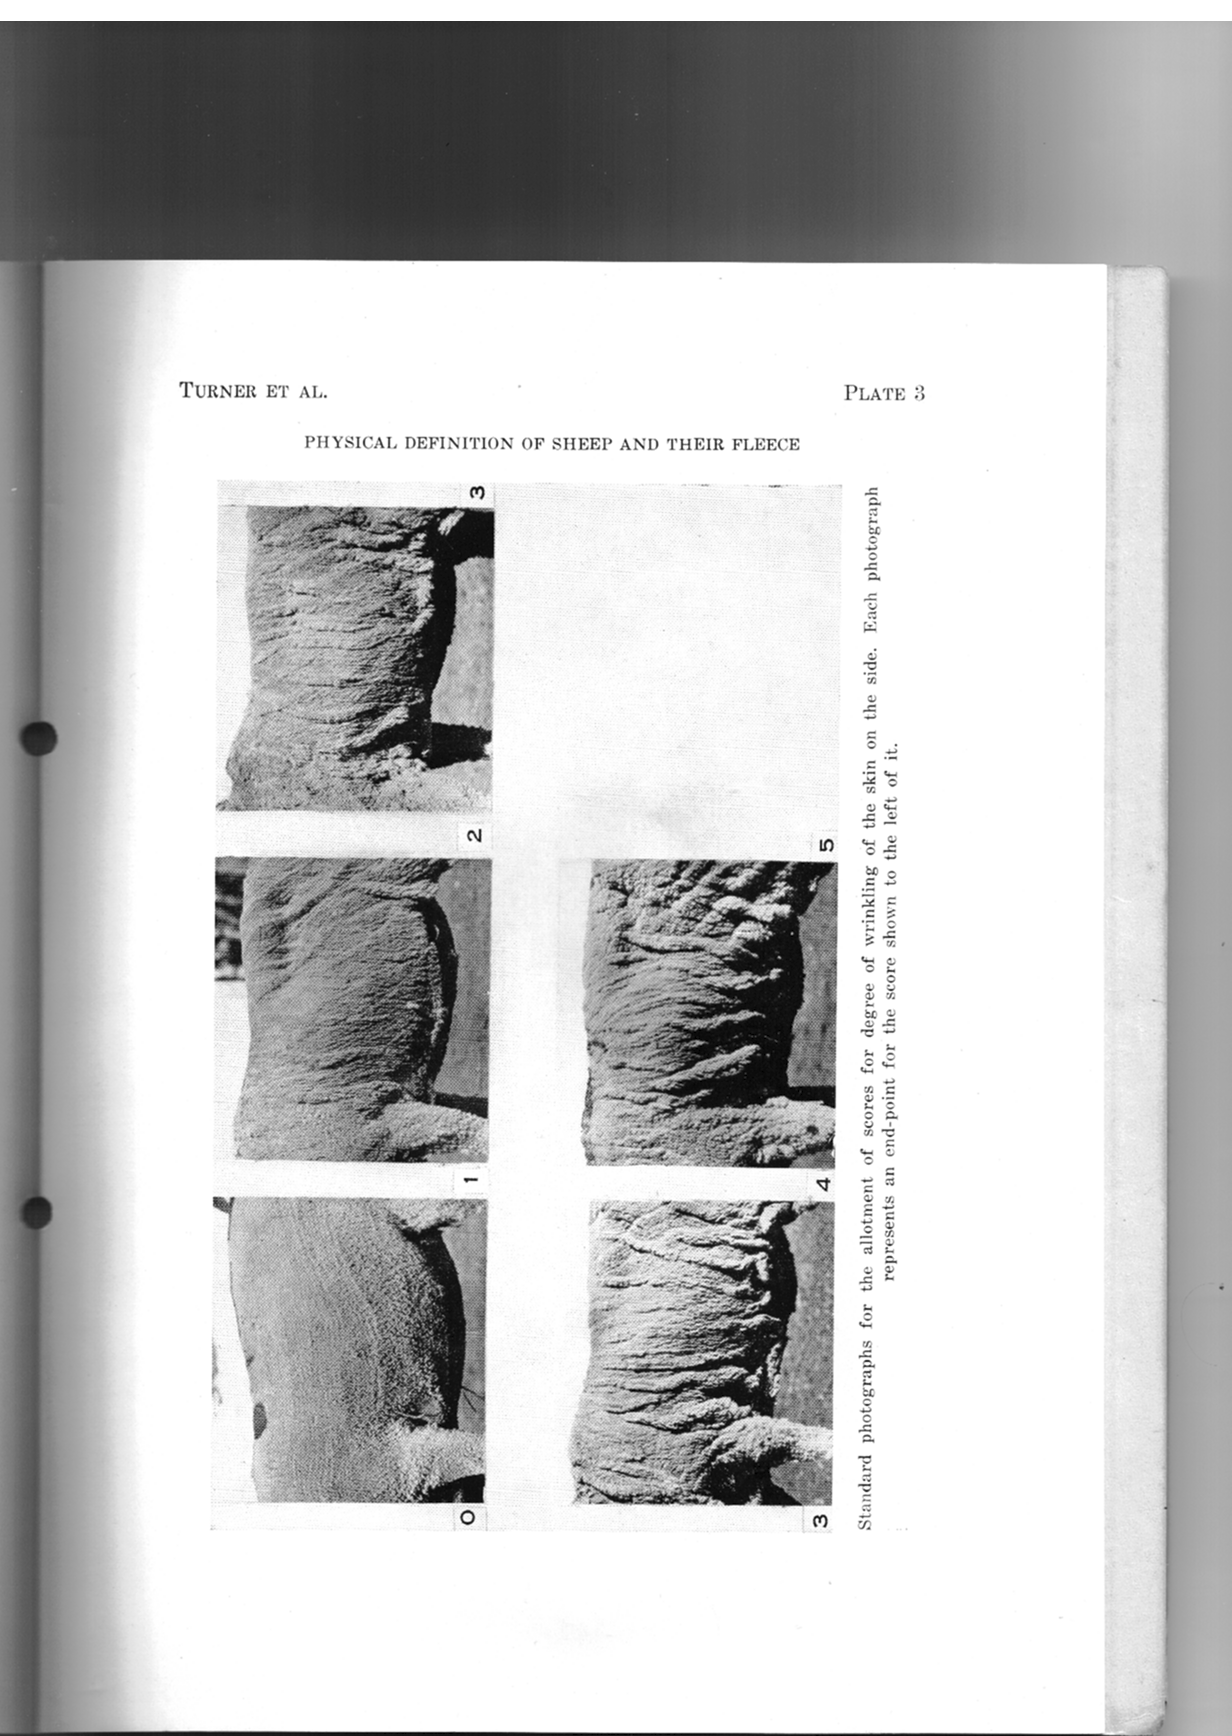
\includegraphics[width=0.9\textwidth]{wrbody.png}
  \caption{Photographic standards for sheep body wrinkle scores from Turner etal(1953)~\cite{turn:53}}
  \label{fig:wrbody}
\end{figure}

%\end{document}


%\documentclass{article}
%\usepackage{graphicx,subfigure}
%\begin{document}

\begin{figure}[!h]
  \centering
   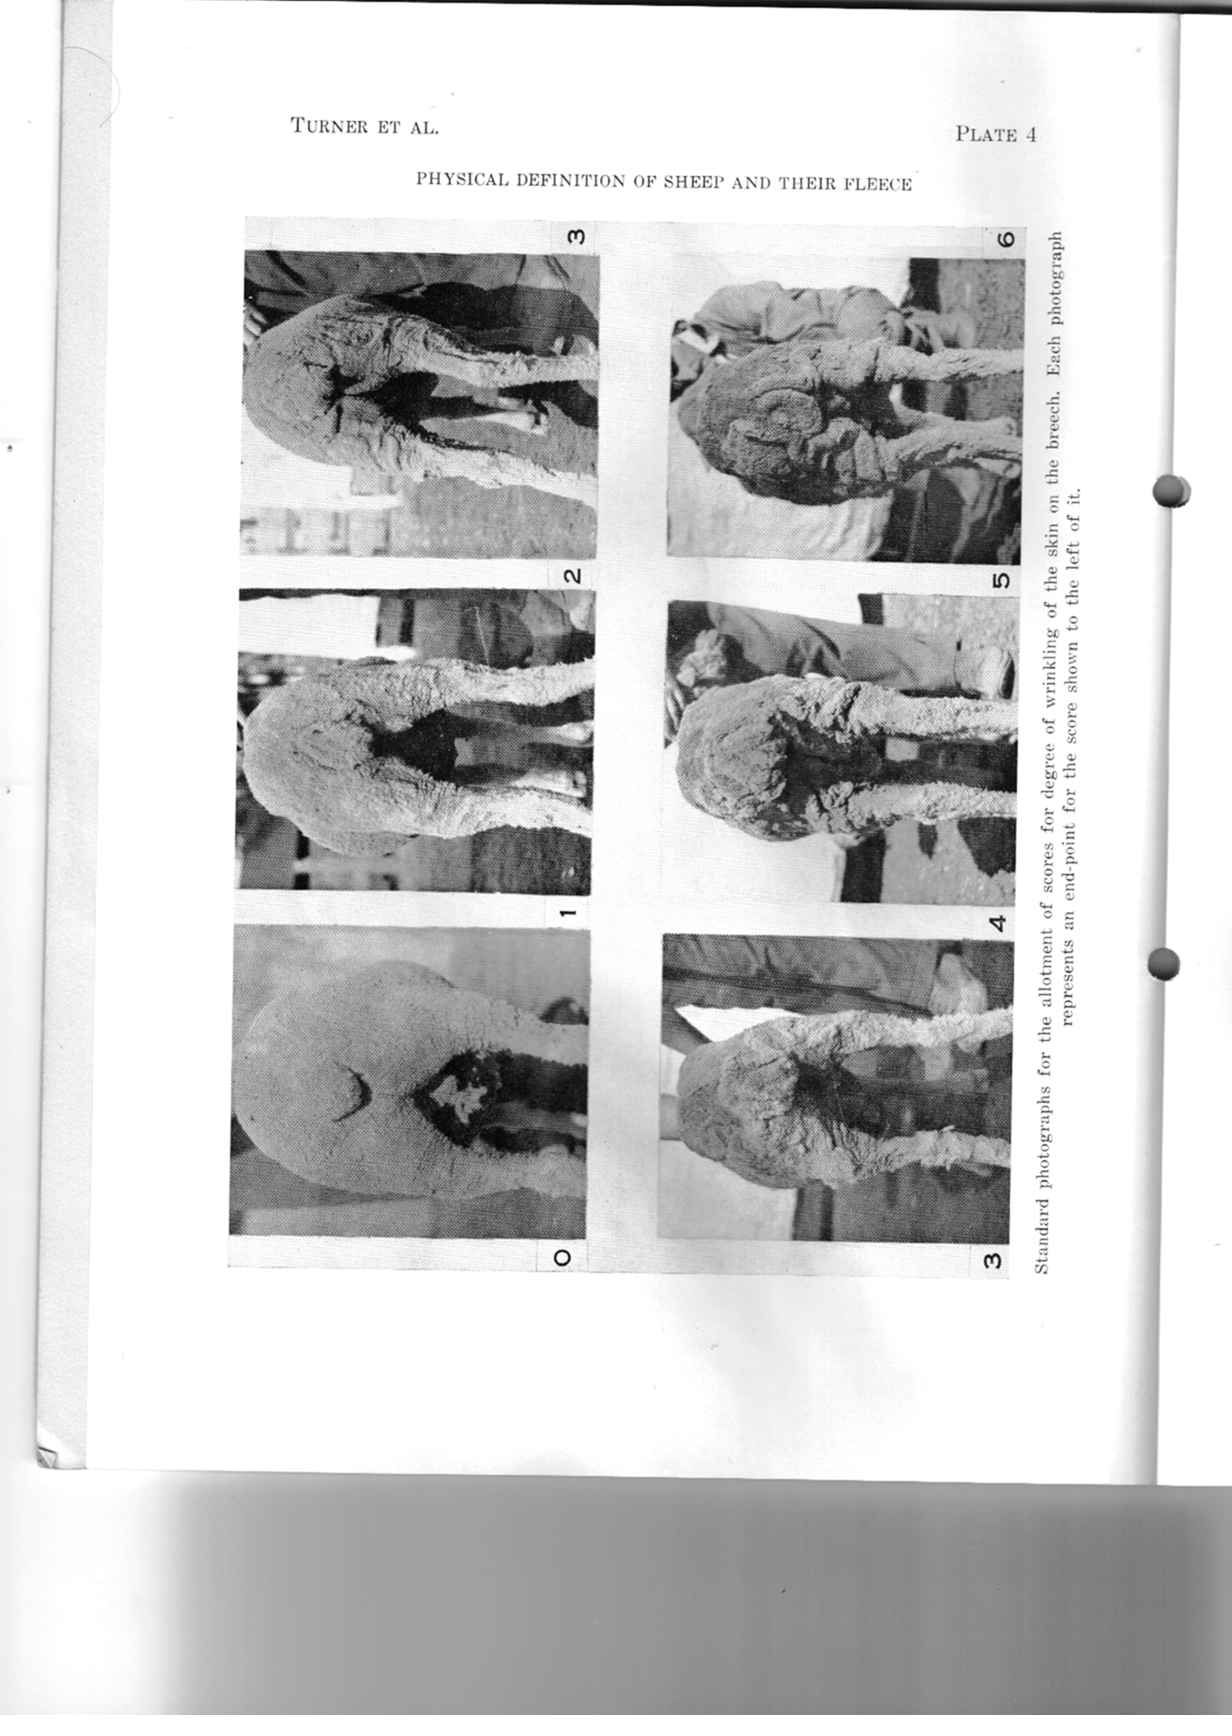
\includegraphics[width=0.9\textwidth]{wrbreech.png}
  \caption{Photographic standards for sheep breech wrinkle scores from Turner etal(1953)~\cite{turn:53}}
  \label{fig:wrbreech}
\end{figure}

%\end{document}


Breech wrinkle scores were not used because the sheep were mulesed. Neck wrinkle scores range from 1 to 6, body wrinkle scores range from 1 to 5, the higher number meaning more wrinkled.  All scores were made at the hogget stage, approximately 12 to 15 months of age, immediately after hogget shearing. Animals were held in a standing position for scoring.
Analyses were also made of an overall wrinkle score which was the total of separate neck and body scores and therefore had a range of 2 to 11. 

All other measurements were as described in Jackson(2017)~\cite{jack:17}, or  in the original papers describing each experiment. The measurements of particular interest in relation to their correlation with wrinkle score are detailed in Table~\ref{tab:measts}
%\documentclass{article}
%\usepackage{lscape,longtable}
%\begin{document}
\begin{center}
\begin{landscape}
\begin{longtable}{p{1.5in}|p{0.8in}|p{1.5in}|p{1.0in}|p{2.5in}}
\caption{Definition of traits measured}  \\
\hline
\label{tab:measts}
    Trait name & Abbreviation  & Units & Age measured  &  Description \\ 
\hline
\endfirsthead
\multicolumn{5}{c}%
{\tablename\ \thetable\ -- \textit{Continued from previous page}} \\
\hline
    Trait name & Abbreviation  & Units & Age measured  &  Description \\ 
\hline
\endhead
\hline
\multicolumn{5}{r}{\textit{Continued on next page}} \\
\endfoot
\hline
\endlastfoot
%\env{longtable}[p{1.5in}|p{0.8in}|p{1.5in}|p{1.0in}|p{2.5in}]
 Staple length & Stal & mm & 14 months & Length of wool staple 10 months growth \\
 Crimp frequency & Crimp & no per 2.5cm & 14 months & Staple crimp frequency\\
 Fibre diameter & Diam & microns & 14 months & Mean fibre diameter by airflow technique \\
 Greasy Fleece Weight & Gfw & Kg & 14 months & Weight of fleece in shearing shed \\
 Yield & Yld & percentage & 14 months & Percent of clean wool in fleece at 16\% regain \\
 Clean wool weight & Cww & Kg & 14 months & Weight of clean fibre at 16\% regain \\
 Bodyweight & Bwt & Kg & 14 months & Live weight of animal \\
 Neck wrinkle & WrN & score 0-6 (0=plain,6=wrinkled) & 14 months & Score for skin wrinkle on neck region \\
 Body wrinkle & WrB & score 0-5 (0=plain,5=wrinkled) & 14 months & Score for skin wrinkle on body region \\
 Total wrinkle & WrT & sum of WrN and WrB & 14 months & Sum of neck and body wrinkle scores \\
 Face cover & Face & score 1-7 (1=open, 7=muffled) & 14 months & Score for wool cover on the face \\
 Follicle number per unit area & Fnua & no per $mm_{2}$ & 14 months & No of primary and secondary follicles per $mm_{2}$ from skin biopsy \\
 Follicle $S/P$ ratio & Fr & no units & 14 months & Ratio of no of primary to no of secondary follicles from skin biopsy \\
  Follicle depth & Fd & mm & 14 months & Average follicle depth from skin biopsy and vertical section \\
  Follicle curvature & Fc & score 1-7 (1=straight, 7=curved) & 14 months & Follicle curvature score from skin biopsy and vertical section \\
  Follicle unevenness & Fu & score 1-5 (1=even, 5=uneven) & 14 months & Score for unevenness of follicle depth from skin biopsy and vertical section \\
  Birth weight & Birwt & Kg & day of birth & Weight of lamb on day of birth \\
  Birthcoat score side & Bcts & score 1-6 (1=no halo hairs on side, 6=fully covered) & day of birth & Score for pattern of halo hairs on side of lamb at day of birth \\
  Birthcoat score back & Bctb & score 1-6 (1=no halo hairs on mid backline, 6=dense halo hairs) & day of birth & Score for density of halo hairs on mid backline on day of birth \\
  Weaning weight & Weanwt & Kg & approx 4 months & Weight of lamb on day of weaning \\
  Mean diameter of primaries & Dp & microns & 14 months & Mean diameter of primary fibres from biopsy and horizontal section \\
  Mean diameter of secondaries & Ds & microns & 14 months & Mean diameter of secondary fibres from biopsy and horizontal section \\
  Mean diameter of primaries and secondaries & Dps & microns & 14 months & Mean diameter of primary and secondary fibres from biopsy and horizontal section \\
  Primary to secondary diameter ratio & DpovDs & no units & 14 months & Ratio of mean diameter of primary fibres to mean diameter of secondary fibres \\

\end{longtable}
\end{landscape}
\end{center}
%\end{document}


\section{Statistical techniques}
\label{sect:stats}
The initial step in analysing these data was to fit a mixed model which adjusted for appropriate fixed effects and estimated additive genetic, environmental, and phenotypic variance components for wrinkle scores. 

In subsequent steps various nonadditive genetic effects were added to the mixed model and their contributions to phenotypic variance estimated.  The reason for doing this sequentially is that nonadditive genetic effects are often  strongly correlated with additive genetic and environmental effects, so one needs to be cautious of introducing confounding into the fitted model.

After finding which effects were important for wrinkle scores, the relationship between wrinkle and some other traits was examined ina multivariate model.

\subsection{Mixed model fitting}
The software used for mixed model fitting and estimation of variance components and genetic parameters is known as {\em dmm}. {\em dmm} is free software available under the GPL licence from the CRAN repository. {\em dmm} runs as a package under the R statistical language~\cite{rprog:13}. {\em dmm} has a comprehensive user's guide (Jackson(2015)~\cite{jack:15b}) which covers the statistical theory used for estimation and a set of worked examples.

Variance component estimation is one of the most difficult areas of statistics. It is comprehensively documented by Searle et al (1992)~\cite{sear:92}. The procedure which current wisdom seems to consider most appropriate is called REML. The procedures used by {\em dmm} are MINQUE and bias-corrected-ML. In most cases where data are not extremely unbalanced, there is very little difference between procedures.  For the current task, {\em dmm} is most suited, because it handles multiple traits with unequal replication, because it estimates both variance/covariance components and genetic parameters arising therefrom, because it allows estimation of maternal as well as individual genetic and environmental variance components and the covariances between them.  {\em dmm} makes extensive use of procedures developed by Wolak(2014)~\cite{wola:14} for computing additive and non-additive relationship matrices .

The procedure followed by {\em dmm} is heirarchical. We first fit a model for fixed effects modelling observations on individual sheep as follows

\begin{equation}
\label{model:fixed}
Y_{ijk} = \mu + Sex_{i} + YearbixLine_{j} + r_{ijk}
\end{equation}

where
\begin{description}
\item[$Y_{ijk}$] is an observation on the kth individual of the ith Sex and the jth Year of birth x Line combination
\item[$\mu$] is an overall mean of the observations
\item[$Sex_{i}$] is an effect due to the ith Sex
\item[$YearbixLine_{j}$] is an effect due to the jth combination of Year of birth and Line
\item[$r_{ijk}$] is a residual deviation for the kth individual of the ith Sex and the jth Year of birth x Line combination
\end{description}

Equation~\ref{model:fixed} is stated as a univariate model for simplicity. It can, of course be fitted to each of a set of traits. The residual deviations from model~\ref{model:fixed} represent the observations {\em adjusted for} the fixed effect.

The next step is to fit a dyadic model to the residuals from model~\ref{model:fixed}. A dyad is a pair of individuals. A dyadic model is a model for the covariances between the residuals for pairs of individuals. The dyadic model attempts to fit various genetic and environmental variance/covariance components to the covariances between the residuals for each dyad. In the present case we first attempt an elementary partitioning of the dyadic covariances into additive genetic and environmental variance/covariance components. The dyadic model for this simple case can be written

\begin{equation}
\label{model:dyadic}
Cov(r_{k},r_{k^{`}}) = A_{kk^{`}} VarG(Ia) + E_{kk^{`}} VarE(I) + \Delta_{kk^{`}}
\end{equation}

where
\begin{description}
\item[$Cov(r_{k},r_{k^{`}})$] is the covariance of the kth and $k^{`}$th residuals from the fitting of model~\ref{model:fixed}
\item[$A_{kk^{`}}$] is the $kk^{`}$th element of the additive genetic relationship matrix, that is the relationship coefficient between the kth and $k^{`}$th individuals
\item[$VarG(Ia)$] is the individual additive genetic variance
\item[$E_{kk^{`}}$] is the $kk^{`}$th element of the environmental relationship matrix which is usually assumed to be an identity matrix
\item[$VarE(I)$] is the individual environmental variance
\item[$\Delta_{kk^{`}}$] is the $k^{`}$th residual for the dyadic model~\ref{model:dyadic}
\end{description}

Again, equation~\ref{model:dyadic} is stated as a univariate model for simplicity, and only the most elementary partitioning into $VarG(Ia)$ and $VarE(I)$ is presented. There is a full exposition in Jackson(2015)~\cite{jack:15b}. 

 The dyadic model~\ref{model:dyadic} represents a set of equations which can be solved by ordinary least squares regression techniques to yield estimates of $VarG(Ia)$  and $VarE(I)$. This yields MINQUE estimates for the two variance components. Given these estimates we can then go back to the monadic model~\ref{model:fixed} and obtain GLS estimates of the fixed effects and residuals. If we then use the GLS residuals in the dyadic model~\ref{model:dyadic} we obtain bias-corrected-ML estimates for the two variance components. There is a full presentation of variance component estimation in Jackson(2015)~\cite{jack:15b}.

Given variance component estimates we can readily transform each component to a heritability (if it is univariate) or to a genetic(or environmental) correlation (if it is a between trait covariance component). These transforms, and the accompanying standard error estimates, are fully covered in Jackson(2015)~\cite{jack:15b}


\subsection{Genetic models}
The simple partitioning of phenotypic (co)variances into additive genetic and environmental (co)variances given in equation~\ref{model:dyadic} is almost always the starting point for quantitative genetic analysis. It should be noted that just beacuse a considerable proportion of the phenotypic (co)variancees come out as additive genetic does not mean that most of the gene effects have to be additive. Dominance and epistatic gene effects also generate some additive genetic variance.  This simple analysis leads to estimates of the following components of variance
\begin{description}
\item[VarG(Ia)] variance genetic individual additive
\item[VarE(I)] variance environmental individual
\item[VarP(I)] variance phenotypic individual
\end{description}
In these analyses $VarE(I)$ is simply the variance not accounted for by additive genetic effects. It is the {\em convention} to call it {\em environmental}. It is actually just the residual unexplained variance, most likely due to random environmental differences between individuals, and measurement or appraisal errors, but could  also include variation due to other components not fitted in this model.

After fitting the above additive model, the following nonadditive and maternal effects were investigated by adding stepwise to the model
\begin{description}
\item[VarG(Ma)] variance genetic maternal additive
\item[VarE(M)] variance environmental maternal
\item[VarG(Ia:a)] variance genetic individual additive x additive epistatic
\item[VarGs(Ia)] variance sexlinked individual additive
\item[VarGs(Ma)] variance sexlinked maternal additive
\item[CovG(Ia,Ma)] covariance genetic individual additive x maternal additive
\item[CovG(Ma,Ia)] covariance genetic maternal additive x individual additive
\item[VarG(Id)] variance genetic individual dominance
\item[VarG(Md)] variance genetic maternal dominance
\item[VarGlm(I)] variance genetic maternal lines (cytoplasmic inheritance)
\item[VarGlp(I)]variance genetic paternal lines (Y chromosomal inheritance)
\end{description}


\section{Results}
\subsection{Wrinkle scores partitioning of variance}
We start with data from AB32 and AB20, and with all three wrinkle scores (WrN, WrB, WrT). The result of fitting the basic model with just additive genetic variance is given in Table~\ref{tab:model1}
%\documentclass{article}
%\usepackage{lscape,longtable}
%\begin{document}
% latex table generated in R 3.4.2 by xtable 1.8-2 package
% Sat Oct 21 21:11:58 2017

\begin{center}
\begin{longtable}{|p{0.6in}|p{0.7in}|p{0.6in}|p{0.6in}|p{0.6in}|p{0.6in}|}
\caption{Estimates of proportion of phenotypic variance (VarP(I)) due to VarE(I)  and VarG(Ia), with standard errors and confidence limits, for neck, body, and total wrinkle scores } \\
\hline
\label{tab:model1}
  Trait  & Component & Estimate & StdErr & CI95lo & CI95hi \\
  \hline
\endfirsthead
\multicolumn{5}{c}%
{\tablename\ \thetable\ -- \textit{Continued from previous page}} \\
\hline
    Trait  & Component & Estimate  & StdErr & CI95lo  &  CI95hi \\
\hline
\endhead
\hline
\multicolumn{5}{r}{\textit{Continued on next page}} \\
\endfoot
\hline
\endlastfoot

  WrN & VarE(I) & 0.599 & 0.013 & 0.574 & 0.623 \\ 
  WrN & VarG(Ia) & 0.401 & 0.013 & 0.377 & 0.426 \\ 
  WrN & VarP(I) & 1.000 & 0.000 & 1.000 & 1.000 \\  \hline
  WrB & VarE(I) & 0.604 & 0.013 & 0.580 & 0.629 \\ 
  WrB & VarG(Ia) & 0.396 & 0.013 & 0.371 & 0.421 \\ 
  WrB & VarP(I) & 1.000 & 0.000 & 1.000 & 1.000 \\  \hline
  WrT & VarE(I) & 0.553 & 0.013 & 0.528 & 0.579 \\ 
  WrT & VarG(Ia) & 0.447 & 0.013 & 0.421 & 0.472 \\ 
  WrT & VarP(I) & 1.000 & 0.000 & 1.000 & 1.000 \\ 
   \hline
\end{longtable}
\end{center}
%\end{document}

The three wrinkle scores are similar in this respect - if this simple model is appropriate, around 40 percent of the phenotypic variance is additive genetic. When we speak about phenotypic variance, we mean variance among individuals within a cohort. A cohort is a group of animals reared under common conditions, such as a drop of lambs all born within a short periond and grazed together. To get phenotypic variance we remove systematic effects by including fixed effects for Sex and Year x Line in the model. The result from fitting these fixed effects is given in Table~\ref{tab:model1aov}
% latex table generated in R 3.4.2 by xtable 1.8-2 package
% Tue Jun 19 20:23:57 2018
\begin{table}[ht]
\label{tab:model1aov}
\centering
\begin{tabular}{lrrrrrr}
  \hline
 & Df & Pillai & approx F & num Df & den Df & Pr($>$F) \\ 
  \hline
(Intercept) & 1 & 0.92 & 13662.10 & 3 & 3580 & 0.0000 \\ 
  Sex & 1 & 0.03 & 41.69 & 3 & 3580 & 0.0000 \\ 
  YbxLi & 39 & 0.26 & 8.69 & 117 & 10746 & 0.0000 \\ 
  Residuals & 3582 &  &  &  &  &  \\ 
   \hline
\end{tabular}
\end{table}


We see that both Sex and combinations of Year of birth and Line have significant effects. It is the residual variance from this analysis of variance which is called phenotypic variance, and it is this residual variance which we partition into random effects VarE(I) and VarG(Ia) in Table~\ref{tab:model1}.

We can also partition the residual or phenotypic covariances between the three wrinkle scores. We do this in Table~\ref{tab:model1corr} not as covariances, but as correlations.
%\documentclass{article}
%\usepackage{lscape,longtable}
%\begin{document}
% latex table generated in R 3.4.2 by xtable 1.8-2 package
% Sat Oct 21 21:11:58 2017

\begin{center}
\begin{longtable}{|p{0.6in}|p{0.7in}|p{0.6in}|p{0.6in}|p{0.6in}|p{0.6in}|}
\caption{Estimates of correlation among wrinkle scores for each component of variance} \\
\hline
\label{tab:model1corr}
  Traits  & Component & Estimate & StdErr & CI95lo & CI95hi \\
  \hline
\endfirsthead
\multicolumn{5}{c}%
{\tablename\ \thetable\ -- \textit{Continued from previous page}} \\
\hline
    Traits  & Component & Estimate  & StdErr & CI95lo  &  CI95hi \\
\hline
\endhead
\hline
\multicolumn{5}{r}{\textit{Continued on next page}} \\
\endfoot
\hline
\endlastfoot

  WrN:WrB & VarE(I) & 0.527 & 0.022 & 0.483 & 0.570 \\ 
  WrN:WrB & VarG(Ia) & 0.949 & 0.017 & 0.916 & 0.981 \\ 
  WrN:WrB & VarP(I) & 0.695 & 0.010 & 0.675 & 0.715 \\  \hline
  WrN:WrT & VarE(I) & 0.851 & 0.011 & 0.828 & 0.981 \\ 
  WrN:WrT & VarG(Ia) & 0.986 & 0.009 & 0.970 & 1.002 \\ 
  WrN:WrT & VarP(I) & 0.907 & 0.005 & 0.897 & 0.917 \\  \hline
  WrB:WrT & VarE(I) & 0.854 & 0.011 & 0.831 & 0.876 \\ 
  WrB:WrT & VarG(Ia) & 0.988 & 0.008 & 0.972 & 1.004 \\ 
  WrB:WrT & VarP(I) & 0.909 & 0.005 & 0.899 & 0.919 \\ 
   \hline
\end{longtable}
\end{center}
%\end{document}

We see that the three wrinkle scores have  very high genetic correlations , but the environmental correlations are not so high. A correlation of 0.527 between WrB and WrN means only 27 percent of the variance in WrN is correlated with WrB, at the environmental level. This is probably because the VarE(I) component includes measurement or scoring errors, and these might be uncorrelated.

We are not going to go through all the tedious steps of testing adding various types of nonadditive or maternal variance components to the model. What we do is present the final model containing all random effects found to be significant and of important magnitude. We simply note those components which were either too confounded to be estimable or too small or insignificant to be included. 

The random effects found to be important are shown, with their estimated proportions of variance, in Table~\ref{tab:modelf}
%\documentclass{article}
%\usepackage{lscape,longtable}
%\begin{document}
% latex table generated in R 3.4.2 by xtable 1.8-2 package
% Sat Oct 21 21:11:58 2017

\begin{center}
\begin{longtable}{|p{0.6in}|p{0.7in}|p{0.6in}|p{0.6in}|p{0.6in}|p{0.6in}|}
\caption{Estimates of proportion of phenotypic variance (VarP(I)) due to  all components found to be significant, with standard errors and confidence limits, for neck, body, and total wrinkle scores } \\
\hline
\label{tab:modelf}
  Trait  & Component & Estimate & StdErr & CI95lo & CI95hi \\
  \hline
\endfirsthead
\multicolumn{5}{c}%
{\tablename\ \thetable\ -- \textit{Continued from previous page}} \\
\hline
    Trait  & Component & Estimate  & StdErr & CI95lo  &  CI95hi \\
\hline
\endhead
\hline
\multicolumn{5}{r}{\textit{Continued on next page}} \\
\endfoot
\hline
\endlastfoot

  WrN & VarE(I) & 0.368 & 0.045 & 0.279 & 0.456 \\ 
  WrN & VarG(Ia) & 0.277 & 0.022 & 0.233 & 0.322 \\ 
  WrN & VarG(Ia:a) & 0.213 & 0.062 & 0.091 & 0.334  \\
  WrN & VarG(Ma) & 0.141 & 0.031 & 0.079 & 0.203  \\
  WrN & VarE(M) & 0.002 & 0.017 & -0.031 & 0.035  \\
  WrN & VarGs(Ia) & 0.006 & 0.008 & -0.009 & 0.022 \\
  WrN & VarGs(Ma) & 0.004 & 0.017 & -0.030 & 0.022 \\
  WrN & CovG(Ia,Ma)  & -0.006 & 0.018 & -0.041 & 0.029 \\
  WrN & CovG(Ma,Ia)  & -0.006 & 0.018 & -0.041 & 0.029 \\
  WrN & VarP(I) & 1.000 & 0.000 & 1.000 & 1.000 \\  \hline

  WrB & VarE(I) & 0.250 & 0.047 & 0.158 & 0.343 \\ 
  WrB & VarG(Ia) & 0.236 & 0.023 & 0.191 & 0.282 \\ 
  WrB & VarG(Ia:a) & 0.372 & 0.064 & 0.245 & 0.498  \\
  WrB & VarG(Ma) & 0.237 & 0.033 & 0.171 & 0.303  \\
  WrB & VarE(M) & 0.001 & 0.017 & -0.033 & 0.035 \\
  WrB & VarGs(Ia) & 0.050 & 0.008 & 0.033 & 0.067 \\
  WrB & VarGs(Ma) & 0.006 & 0.018 & -0.029 & 0.042 \\
  WrB & CovG(Ia,Ma) & -0.077 & 0.018 & -0.115 & -0.040 \\
  WrB & CovG(Ma,Ia) & -0.077 & 0.018 & -0.115 & -0.040 \\
  WrB & VarP(I) & 1.000 & 0.000 & 1.000 & 1.000 \\  \hline

  WrT & VarE(I) & 0.251 & 0.045 & 0.161 & 0.340 \\ 
  WrT & VarG(Ia) & 0.285 & 0.022 & 0.241 & 0.329 \\ 
  WrT & VarG(Ia:a) & 0.301 & 0.062 & 0.179 & 0.422  \\
  WrT & VarG(Ma) & 0.224 & 0.032 & 0.160 & 0.287  \\
  WrT & VarE(M)  & 0.000 & 0.001 & -0.001 & 0.001 \\
  WrT & VarGs(Ia) & 0.024 & 0.008 & 0.007 & 0.040 \\
  WrT & VarGs(Ma) & 0.000 & 0.015 & -0.030 & 0.031 \\
  WrT & CovG(Ia,Ma) & -0.043 & 0.017 & -0.078 & -0.007 \\
  WrT & CovG(Ma,Ia) & -0.043 & 0.017 & -0.078 & -0.007 \\
  WrT & VarP(I) & 1.000 & 0.000 & 1.000 & 1.000 \\ 
   \hline
\end{longtable}
\end{center}
%\end{document}

The dominance variance components VarG(Id) and VarG(Md) were found to be very highly correlated, in this dataset, with the environmental variance components VarE(I) and VarE(M) respectively. The actual correlations were 0.985 and 0.998 respectively. This means that is these data, dominance variance is inseparable from environmental variance. We therefore had to omit VarG(Id) and VarG(Md) from the fitted model. There may be dominance effects, but we could not separate them from environmental effects with these data.  That is not unusual in pedigrees with a low level of inbreeding.

Also omitted were the  maternal epistatic component VarG(Ma:a), and the variances between male and female founder lines, VarGlm(I) and VarGlp(I). These were omitted because the estimates were extremely small ( less than $10^{-5}$ ). There was therefore no evidence of maternal additive x additive epistatic effects. and no evidence of either cytoplasmic inheritance ( VarGlm(I)) or paternal Y chromosomal inheritance (VarGlm(I)).

Because the dominance effects were confounded , we were also unable to look at epistatic variance components involving dominance ( VarG(Ia:d), VarG(Id:d) and their maternal equivalents). 

That leaves us with the effects listed in Table~\ref{tab:modelf}. A number of these are also quite small proportions of the phenotypic variance. We could omit VarE(M), VarGs(Ia), VarGs(Ma), CovG(Ia,Ma), and CovG(Ma,Ia) and we would be ignoring only about 10 percent of phenotypic variance. Thus there is little evidence for sexlinked genetic effects, either individual or maternal, and only a tiny (negative) covariance of individual and maternal additive genetic effects.

We are left with VarE(I), VarG(Ia), VarG(Ia:a), and VarG(Ma), and these each account for roughly 1/4 each of the phenotypic variance. Thus there is evidence for additive genetic variance (VarG(Ia)), additive x additive epistatic interaction variance ( VarG(Ia:a)), and maternal additive genetic variance ( VarG(Ma)). 

As a final check we ran the model fit once more, with just the above 4 components of variance included. This is shown in Table~\ref{tab:model4c}
%\documentclass{article}
%\usepackage{lscape,longtable}
%\begin{document}
% latex table generated in R 3.4.2 by xtable 1.8-2 package
% Sat Oct 21 21:11:58 2017

\begin{center}
\begin{longtable}{|p{0.6in}|p{0.7in}|p{0.6in}|p{0.6in}|p{0.6in}|p{0.6in}|}
\caption{Estimates of proportion of phenotypic variance (VarP(I)) due to  the four most significant components, with standard errors and confidence limits, for neck, body, and total wrinkle scores } \\
\hline
\label{tab:model4c}
  Trait  & Component & Estimate & StdErr & CI95lo & CI95hi \\
  \hline
\endfirsthead
\multicolumn{5}{c}%
{\tablename\ \thetable\ -- \textit{Continued from previous page}} \\
\hline
    Trait  & Component & Estimate  & StdErr & CI95lo  &  CI95hi \\
\hline
\endhead
\hline
\multicolumn{5}{r}{\textit{Continued on next page}} \\
\endfoot
\hline
\endlastfoot

  WrN & VarE(I) & 0.400 & 0.050 & 0.301 & 0.498 \\ 
  WrN & VarG(Ia) & 0.313 & 0.024 & 0.266 & 0.360 \\ 
  WrN & VarG(Ia:a) & 0.262 & 0.069 & 0.125 & 0.398  \\
  WrN & VarG(Ma) & 0.025 & 0.010 & 0.005 & 0.045  \\ \hline

  WrB & VarE(I) & 0.278 & 0.050 & 0.179 & 0.378 \\ 
  WrB & VarG(Ia) & 0.252 & 0.024 & 0.205 & 0.300 \\ 
  WrB & VarG(Ia:a) & 0.439 & 0.070 & 0.302 & 0.578  \\
  WrB & VarG(Ma) & 0.029 & 0.010 & 0.008 & 0.049  \\ \hline

  WrT & VarE(I) & 0.273 & 0.051 & 0.173 & 0.373 \\ 
  WrT & VarG(Ia) & 0.318 & 0.024 & 0.271 & 0.366 \\ 
  WrT & VarG(Ia:a) & 0.374 & 0.070 & 0.237 & 0.512  \\
  WrT & VarG(Ma) & 0.033 & 0.010 & 0.012 & 0.053  \\ \hline
\end{longtable}
\end{center}
%\end{document}

We see that the proportions of variance attributed to VarE(I), VarG(Ia), and  VarG(Ia:a) have remained similar, but the proportion of variance attributed to VarG(Ma) is less.  So we confirm the epistatic component but there is some doubt attached to the size of the maternal genetic component.  This sort of shifting around often happens when small but correrlated components are removed from a model. Notice that the standard errors in Table~\ref{tab:model4c} are larger than in Table~\ref{tab:modelf}; there is more unexplained variation. The most reliable estimates are those of Table~\ref{tab:modelf} with all significant components fitted. 

We started this investigation expecting to find some maternal effects on wrinkle, and we have found some, but they are small in terms of proportion of variance. Some genes carried by the mother affect the development of the wrinkle phenotype of the offspring. 

What we did not expect was such a large epistatic component. There are some pairs genes at separate loci which combine to produce a greater effect on wrinkle than would be expected by adding the effects of the two genes alone. This sort of gene action accounts for 21 percent of phenotypic variance in neck wrinkle (WrN) and 37 percent of phenotypic variance in body wrinkle (WrB). There are consequences for breeding and selection. Gains made by selecting epistatic combinations of genes are not permanent, they disappear when the genes segregate.

We have conducted a number of further checks on this analysis. These are presented in Appendix B. In particular we wanted to see if the estimate of VarG(Ia:a), the epistatic component, had been biased in some way. We found nothing. We have to conclude that the epistatic variance for wrinkle score is real and large.


%\subsection{Wrinkle scores and wool crimp}
%\subsection{Wrinkle scores and follicle curvature}
%\subsection{Wrinkle scores and S/P ratio}
%\subsection{Wrinkle scores and diameter of primary fibres}

\section{Discussion}
Maternal genetic effects on wrinkle  have a ready made explanation, but the details of proof are not yet at hand. Mothers with a genetically high wrinkle score are deficient in temperature regulation . Poor temperature regulation may affect foetal skin development ( there is evidence of adverse effects on neural system and developmental disorders in mice, and evidence of adverse effects on lamb mortality in sheep). So 14 percent of phenotypic variance for neck wrinkle, and 24 percent for body wrinkle, being additive genetic maternal is not unexpected.  It supports the above explanation, but we have a long way to go finding all the biological evidence.

Epistatic genetic effects on wrinkle are another matter. We did not expect this, but we should have, because it strongly supports our current theory about the way that wrinkles are formed.  The supporting evidence is still being assembled, but briefly, wrinkles form because there are two layers in the skin of the developing lamb foetus which expand at different rates. These are the papillary layer containing the wool follicles, and the layer of dermis immediately below the follicle bulbs which can contain varying amounts of collagen fibril development. When a lot of follicles initiate they expand the upper dermis considerably (Jackson and Watts (2018)~\cite{jack:18}). When a lot of collagen fibrils form in the dermis below follicle bulbs, it binds the dermis against expansion and may even shrink it (Watts personal communication). The conflict between these two tensions causes the epidermis and dermis to fold, just like a bimetal strip bending. Only sheep with both a high follicle number and a high collagen develop wrinkle. That is where the interaction or epistatic effect is coming from. The genes for follicle number interact with the genes for collagen development.  That is what causes epistatic effects - two sets of genes interacting.

The other issue that complicates this interpretation is that not all epistatic gene effects appear as epistatic variance when we do a partitioning of phenotypic variation. Some of them do, and some appear in the additive genetic variance. So the 27 percent of additive genetic variance for neck wrinkle ( and 24 percent for body wrinkle) may also be  at least in part a reflection of epistatic gene action. Our wrinkle theory actually says that all the variation in wrinkle is controlled by interaction between follicle number and collagen amount, so it is possible that all the variance analysed as additive genetic is actually due to interaction, as well as all that actually analysed as epistatic, and in that case we are looking at 50 percent of the phenotypic variance supporting our theory. That is a phenomenally successful result. 

We tried to show, using a covariance analysis, that some traits which we regarded as indicators of the two interacting components of wrinkle , could 'explain' some of the epistatic variance. This was only partly successful. It is shown in Appendix A. There were too many analysis difficulties for it to be definitive.

We conclude with a quotation from Lynch and Walsh(1997)~\cite{lync:97}
\begin{quote}
 Because of the heirarchical way in which genetic effects are defined, we might expect the magnitude of genetic variance components to become progressively smaller at higher stages in the heirarchy. Indeed, it is common for quantitative geneticists to use this argument as a rationalization for ignoring epistasis altogether. Unfortunately, such logic does not always hold up -- as pointed out in the previous chapter, unless information on gene frequencies is available, variance components provide limited insight into the physiological mode of gene action.
\end{quote}
That says it all.

\appendix
\section{Appendix - can covariance analyses confirm the epistasis explanation?}
We have asserted that the reason why wrinkle score has a large epistatic variance component is that wrinkle is determined by two interacting components. We have tentatively identified these components as
\begin{description}
\item[dermal expansion due to follicle development] in particular the development of large numbers of secondary derived follicles at around day 100 of gestation results in an expansion of the upper dermis relative to other skin layers
\item[dermal binding or contraction due to collagen development] in particular  the development of a layer of non reticular collagen below the follicle bulbs in the dermis prevents dermal expansion and may even lead to contraction
\end{description}
We suggest it is the tension between these two components which leads to skin folding.

One way of checking  this explanation of epistasis is to find some measures of the two components of wrinkle, to remove their effect on wrinkle using covariance analysis, and to see if the variance of 'covariance adjusted wrinkle score'  is still epistatic. For the follicle development factor we really need a measure of the number of secondary derived or branching follicles. We do not have these data. The best we can do is S/P ratio ( Fr ) or diameter of primary follicles (Dp). For collagen development we have no direct measure at all. We do know , however, that one strong side effect of collagen development is follicle curvature (Fc), so we propose to use Fc, and its wool effect crimp frequency (Crimp).

We did these covariance analyses one trait at a time. So we have one analysis of WrN unadjusted, one analysis of WrN/Fr ( wrinkle adjusted for Fr), one analysis of WrN/Dp, one analysis of WrN/Crimp, and one analysis of WrN/Fc. The result is shown in Figure~\ref{fig:wrncov}
%\documentclass{article}
%\usepackage{graphicx,subfigure}
%\begin{document}

\begin{figure}[!h]
  \centering
   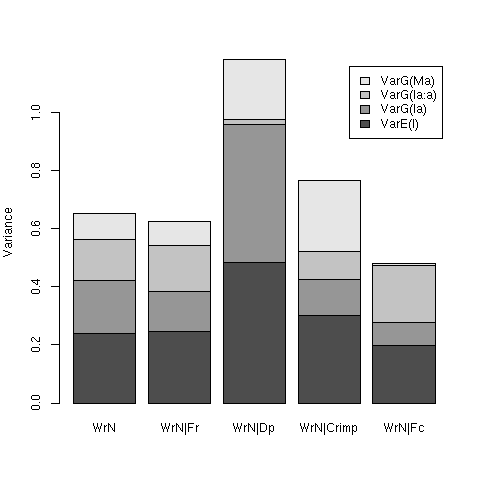
\includegraphics[width=0.9\textwidth]{wrncov.png}
  \caption{Variance component analyses of neck wrinkle scores (WrN)  unadjusted and adjusted for each of the four component indicators (Fr, Dp, Crimp, Fc) in turn}
  \label{fig:wrncov}
\end{figure}

%\end{document}


Then we repeat the whole thing for WrB, with result shown in Figure~\ref{fig:wrbcov}
%\documentclass{article}
%\usepackage{graphicx,subfigure}
%\begin{document}

\begin{figure}[!h]
  \centering
   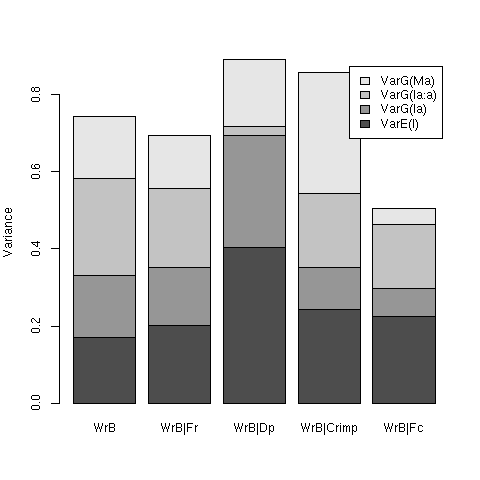
\includegraphics[width=0.9\textwidth]{wrbcov.png}
  \caption{Variance component analyses of body wrinkle scores (WrB)  unadjusted and adjusted for each of the four component indicators (Fr, Dp, Crimp, Fc) in turn}
  \label{fig:wrbcov}
\end{figure}

%\end{document}


We see that for both WrN and WrB, the only adjustment that substantially reduced the epistatic variance was Dp. For body wrinkle Fr, Crimp and Fc adjustment also reduced epistatic variance slightly. For neck wrinkle, epistatic variance was not as large unadjusted, and only Dp adjustment led to further  reduction.

There were a number of difficulties with these covariance analyses.  The numbers of degrees of freedom changed substantially when the covariance adjustments were added, due to missing data for the covariates.  We have only shown the four most significant components in Figures~\ref{fig:wrncov} and ~\ref{fig:wrbcov}, the remaining five components also varied with adjustment. The total phenotypic variance tended to increase with adjustment in some cases, this being a reflection of added measurement errors. One would expect, that everything else being equal, the phenotypic variance would be less for an adjusted variable, than for unadjusted. 

So what can we conclude from this exercise? For body wrinkle there is some evidence that covariance adjustment removes some of the epistasis. For neck wrinkle it is less clear, and the epistatic component was smaller anyway for neck wrinkle. It may be that neck folds have an additional component that we have not identified. 

Why was the adjustment using Dp succesful in removing epistatic variance? Well Dp is a powerful indicator of ability to develop masses of secondary derived follicles. The other 3 indicators are less direct. In particular, Fc and Crimp are side effects of collagen development, and not all the variation in Fc and Crimp is due to collagen, some being due to intrinsic curvature of the fibre.  Fr includes So follicles as well as Sd, so it is also influenced by extraneous factors. We simply do not have direct accurate measures of branching follicle development or of collagen development.

\section{Appendix - checks on the variance component analyses}
\subsection{Omitted variable bias}
Variance component analyses are not straightforward. In a mixed model, when partitioning the phenotypic variance into components, one needs to be extremely careful that one does not omit some component that is both large and significant. To do so would bias the estimates for all components. One can see this by comparing Tables~\ref{tab:model1} and ~\ref{tab:model4c} from the Results section. When only VarE(I) and VarG(Ia) are partitioned, these account for about 60 percent and 40 percent of the phenotypic variance. When VarG(Ia:a) and VarG(Ma) are also fitted, the four components each account for about 25 percent of the phenotypic variance. So the heritability has 'shrunk' from 40 percent top 25 percent. The 40 percent estimate is substantially wrong. It is biased because not all important components were fitted.

So we need to be sure that our 4 component partitioning has not ignored some other effect that is large and significant. In the Results section we note that  there were some components (VarG(Id) and VarG(Md) ) which were too highly correlated with other components to be separately estimable. We also noted that VarG(Ma:a), VarGlm(I) and VarG(lp(I) were absolutely tiny and could be safely omitted. THen there were 5 components (VarE(M), VarGs(Ia), VarGs(Ma), CovG(Ia,Ma), and CovG(Ma,Ia))  which were quite small but not zero, and could also be omitted.

What we have not checked is environmental cross-effect covariances. In particular CovE(I,M) and CovE(M,I) need to be examined. We ran another analysis partitioning the phenotypic variance into 9 components (VarE(I), VarG(Ia) , VarG(Ia:a), VarE(M), VarG(Ma), CovG(Ia,Ma), CovG(Ma,Ia), CovE(I,M), CovE(M,I)), so that all possible cross effect covariances were included). The estimates for CovE(I,M) and CovE(M,I) were tiny, and the other components did not shift around significantly. We conclude that cross effect covariances are not an issue, and can be ignored.

\subsection{Maximum likelihood estimates}
Another way of checking is to use a different estimation technique. The package {\em dmm} can also do bias-corrected maximum likelihood estimates. This is an iterative procedure in which the fixed effects are iterated towards GLS estimates, using successively improved estimates of the variance components. 

The results of a bias-corrected ML iteration are given in Table~\ref{tab:model4cgls}
%\documentclass{article}
%\usepackage{lscape,longtable}
%\begin{document}
% latex table generated in R 3.4.2 by xtable 1.8-2 package
% Sat Oct 21 21:11:58 2017

\begin{center}
\begin{longtable}{|p{0.6in}|p{0.7in}|p{0.6in}|p{0.6in}|p{0.6in}|p{0.6in}|}
\caption{Bias-corrected maximum likelihood estimates of proportion of phenotypic variance (VarP(I)) due to  the four most significant components, with standard errors and confidence limits, for neck, body, and total wrinkle scores } \\
\hline
\label{tab:model4cgls}
  Trait  & Component & ML Estimate & StdErr & CI95lo & CI95hi \\
  \hline
\endfirsthead
\multicolumn{5}{c}%
{\tablename\ \thetable\ -- \textit{Continued from previous page}} \\
\hline
    Trait  & Component & ML Estimate  & StdErr & CI95lo  &  CI95hi \\
\hline
\endhead
\hline
\multicolumn{5}{r}{\textit{Continued on next page}} \\
\endfoot
\hline
\endlastfoot

  WrN & VarE(I) & 0.343 & 0.028 & 0.268 & 0.399 \\ 
  WrN & VarG(Ia) & 0.269 & 0.013 & 0.242 & 0.295 \\ 
  WrN & VarG(Ia:a) & 0.351 & 0.039 & 0.274 & 0.429  \\
  WrN & VarG(Ma) & 0.035 & 0.005 & 0.024 & 0.046  \\ \hline

  WrB & VarE(I) & 0.228 & 0.029 & 0.169 & 0.286 \\ 
  WrB & VarG(Ia) & 0.195 & 0.013 & 0.168 & 0.221 \\ 
  WrB & VarG(Ia:a) & 0.530 & 0.040 & 0.450 & 0.609  \\
  WrB & VarG(Ma) & 0.046 & 0.006 & 0.035 & 0.058  \\ \hline

  WrT & VarE(I) & 0.226 & 0.030 & 0.167 & 0.248 \\ 
  WrT & VarG(Ia) & 0.257 & 0.013 & 0.230 & 0.284 \\ 
  WrT & VarG(Ia:a) & 0.467 & 0.040 & 0.387 & 0.547  \\
  WrT & VarG(Ma) & 0.049 & 0.006 & 0.037 & 0.060  \\ \hline
\end{longtable}
\end{center}
%\end{document}

Table~\ref{tab:model4cgls} should be compared with Table~\ref{tab:model4c} which are the MINQUE estimates with OLS estimates of fixed effects. 

We see that the epistatic component (VarG(Ia:a)) has actually increased in Table~\ref{tab:model4cgls} compared to Table~\ref{tab:model4c}, and the standard errors of estimates are smaller. The iterative estimation procedure only took 3 rounds to converge - the output is shown below
\begin{verbatim}
.....
GLS-b step:
Warning: Multivariate GLS is not same as multiple univariate GLS's
Round =  1  Stopcrit =  0.06876087 
Round =  2  Stopcrit =  0.01187422 
Round =  3  Stopcrit =  0.002260546 
Iteration completed - count =  3 
Convergence achieved
GLS-b step completed successfully:
....
\end{verbatim}
This is a very well behaved iteration. It is a matter of experience that this iteration will misbehave if the model is not appropriate for the data. This is an indication that our estimate of epistatic variance ( and the other 3 components) is free of interfering issues with the model or data.

\subsection{Outlier effects}
It is possible for analyses to be biased by presence of a small number of outliers. The package {\em dmm} has an option to use robust regression methods instead of ordinary least squares for variance component estimation. This is possible because {\em dmm} reduces variance component estimation to a regression problem.

We reran the analysis from Table~\ref{tab:model4c}  using robust regression. Robust regression is a univariate procedure. We had to do one trait at a time. W
e only did WrN and WrB. That was sufficient to achieve our aim of looking at out
lier bias. The results are shown in Table~\ref{tab:model4crob}
%\documentclass{article}
%\usepackage{lscape,longtable}
%\begin{document}
% latex table generated in R 3.4.2 by xtable 1.8-2 package
% Sat Oct 21 21:11:58 2017

\begin{center}
\begin{longtable}{|p{0.6in}|p{0.7in}|p{0.6in}|p{0.6in}|p{0.6in}|p{0.6in}|}
\caption{Robust regression estimates of proportion of phenotypic variance (VarP(I)) due to  the four most significant components, with standard errors and confidence limits, for neck,  and body wrinkle scores } \\
\hline
\label{tab:model4crob}
  Trait  & Component & Estimate & StdErr & CI95lo & CI95hi \\
  \hline
\endfirsthead
\multicolumn{5}{c}%
{\tablename\ \thetable\ -- \textit{Continued from previous page}} \\
\hline
    Trait  & Component & Estimate  & StdErr & CI95lo  &  CI95hi \\
\hline
\endhead
\hline
\multicolumn{5}{r}{\textit{Continued on next page}} \\
\endfoot
\hline
\endlastfoot

  WrN & VarE(I) & 0.311 & 0.110 & 0.094 & 0.527 \\ 
  WrN & VarG(Ia) & 0.327 & 0.052 & 0.224 & 0.431 \\ 
  WrN & VarG(Ia:a) & 0.340 & 0.153 & 0.039 & 0.640  \\
  WrN & VarG(Ma) & 0.021 & 0.022 & -0.023 & 0.065  \\ \hline

  WrB & VarE(I) & 0.123 & 0.109 & -0.091 & 0.338 \\ 
  WrB & VarG(Ia) & 0.152 & 0.051 & 0.051 & 0.254 \\ 
  WrB & VarG(Ia:a) & 0.668 & 0.152 & 0.368 & 0.967  \\
  WrB & VarG(Ma) & 0.055 & 0.022 & 0.011 & 0.099  \\ \hline

\end{longtable}
\end{center}
%\end{document}

The resuts are similar, slight decreases in VarE((I) and VarG(Ia), and sligtht increases in VarG(Ia:a) and VarG(Ma). Standard errors are larger, because some observations have been discarded by the robust regression procedure. 

So there is strong evidence that our analysis showing epistatic variance was not  biased by outlier effects. 

\subsection{Correlation between estimates}
The components we have chosen to include in our partitioning of phenotypic variance are correlated with one another. Table~\ref{tab:corre9} shows correlations among the columns of the coefficient matrix $W$ for the 9 compoonents included in Table~\ref{tab:modelf}.
% latex table generated in R 3.4.2 by xtable 1.8-2 package
% Thu Jul 12 20:06:00 2018
\begin{landscape}
\begin{table}[ht]
\centering
\caption{Correlations among columns of the $W$ matrix used to estimate 9 components of variation in wrinkle scores}
\label{tab:corre9}
\begin{tabular}{rrrrrrrrrr}
  \hline
 & VarE(I) & VarG(Ia) & VarG(Ia:a) & VarG(Ma) & VarE(M) & VarGs(Ia) & VarGs(Ma) & CovG(Ia,Ma) & CovG(Ma,Ia) \\ 
  \hline
VarE(I) & 1.00 & 0.54 & 0.89 & 0.50 & 0.60 & 0.53 & 0.42 & 0.35 & 0.35 \\ 
  VarG(Ia) & 0.54 & 1.00 & 0.82 & 0.55 & 0.50 & 0.67 & 0.50 & 0.59 & 0.59 \\ 
  VarG(Ia:a) & 0.89 & 0.82 & 1.00 & 0.60 & 0.63 & 0.68 & 0.52 & 0.53 & 0.53 \\ 
  VarG(Ma) & 0.50 & 0.55 & 0.60 & 1.00 & 0.82 & 0.64 & 0.93 & 0.76 & 0.76 \\ 
  VarE(M) & 0.60 & 0.50 & 0.63 & 0.82 & 1.00 & 0.53 & 0.70 & 0.57 & 0.57 \\ 
  VarGs(Ia) & 0.53 & 0.67 & 0.68 & 0.64 & 0.53 & 1.00 & 0.65 & 0.61 & 0.61 \\ 
  VarGs(Ma) & 0.42 & 0.50 & 0.52 & 0.93 & 0.70 & 0.65 & 1.00 & 0.71 & 0.71 \\ 
  CovG(Ia,Ma) & 0.35 & 0.59 & 0.53 & 0.76 & 0.57 & 0.61 & 0.71 & 1.00 & 0.58 \\ 
  CovG(Ma,Ia) & 0.35 & 0.59 & 0.53 & 0.76 & 0.57 & 0.61 & 0.71 & 0.58 & 1.00 \\ 
   \hline
\end{tabular}
\end{table}
\end{landscape}


The correlations of sufficient magnitude to be of concern are between VarE(I) and VarG(Ia:a) ( 0.89), and between VarG(Ia) and VarG(Ia:a) ( 0.82). Because these involve the major components of interest, we need to look further. 

We reran the analysis from Table~\ref{tab:modelf} using principal component regression instead of OLS. There were 9 variance components estimated, so we are talking about estimation in a 9-dimensional parameter space. Of these 9 dimensions, the principal component regression showed that only about 5 dimensions were significant. This conclusion is reached by examination of the proportins of variance explained by successively increasing numbers of principal components. This is shown in Table~\ref{tab:pccumvar}
%\documentclass{article}
%\usepackage{lscape,longtable}
%\begin{document}
% latex table generated in R 3.4.2 by xtable 1.8-2 package
% Sat Oct 21 21:11:58 2017

\begin{center}
\begin{longtable}{|p{2.0in}|p{2.0in}|}
\caption{Cumulative proportions of variance accounted for by successively increasing numbers of principal components in a principal component regression analysis of wrinkle score data} \\
 \hline
\label{tab:pccumvar}
  Number of  Principal Components & Percent variance explained \\
  \hline
\endfirsthead
\multicolumn{2}{c}%
{\tablename\ \thetable\ -- \textit{Continued from previous page}} \\
 \hline
    Number of  Principal Components & Percent variance explained  \\
\hline
\endhead
\hline
\multicolumn{2}{r}{\textit{Continued on next page}} \\
\endfoot
\hline
\endlastfoot

 1 & 70.03 \\
 2 & 82.06 \\
 3 & 88.48 \\
 4 & 92.76 \\
 5 & 95.60 \\
 6 & 97.90 \\
 7 & 99.38 \\
 8 & 99.88 \\
 9 & 100.00 \\ 
   \hline
\end{longtable}
\end{center}
%\end{document}


What happens in principal component regression is that the regression coefficients are estimated by regressing the data on the set of 9 ( or fewer) principal components, rather than on the 9 variance component parameters of interest. This has the feature that the 9 components are independent, so the problem with correlations, noted above, disappears. We can then take the principal component regression coefficients, and convert them back to variance component estimates, ie to regressions on the original X variates, which in our case are columns of the W matrix. If we do this using all 9 principal components, we get exactly the same estimates of variance components as we get using OLS. The interest is in using fewer than 9 principal components, in the present case about 5 should be adequate.

The variance component parameter estimates we get using 5 principal components are shown in Table~\ref{tab:modelfpc5}.
%\documentclass{article}
%\usepackage{lscape,longtable}
%\begin{document}
% latex table generated in R 3.4.2 by xtable 1.8-2 package
% Sat Oct 21 21:11:58 2017

\begin{center}
\begin{longtable}{|p{0.6in}|p{0.7in}|p{0.6in}|p{0.6in}|p{0.6in}|p{0.6in}|}
\caption{Estimates of proportion of phenotypic variance (VarP(I)) due to  nine variance components of Table~\ref{tab:modelf}, but estimated by principal component regression using only 5 principal components. With standard errors and confidence limits, for neck, body, and total wrinkle scores } \\
\hline
\label{tab:modelfpc5}
  Trait  & Component & Estimate & StdErr & CI95lo & CI95hi \\
  \hline
\endfirsthead
\multicolumn{5}{c}%
{\tablename\ \thetable\ -- \textit{Continued from previous page}} \\
\hline
    Trait  & Component & Estimate  & StdErr & CI95lo  &  CI95hi \\
\hline
\endhead
\hline
\multicolumn{5}{r}{\textit{Continued on next page}} \\
\endfoot
\hline
\endlastfoot

  WrN & VarE(I) & 0.185 & 0.005 & 0.174 & 0.196 \\ 
  WrN & VarG(Ia) & 0.326 & 0.007 & 0.312 & 0.339 \\ 
  WrN & VarG(Ia:a) & 0.231 & 0.002 & 0.225 & 0.236  \\
  WrN & VarG(Ma) & 0.018 & 0.002 & 0.013 & 0.023  \\
  WrN & VarE(M) & 0.164 & 0.008 &  0.147 & 0.180  \\
  WrN & VarGs(Ia) & 0.002 & 0.004 & 0.016 & 0.033 \\
  WrN & VarGs(Ma) & 0.000 & NA & NA & NA \\
  WrN & CovG(Ia,Ma)  & 0.024 & 0.014 & -0.004 & 0.053 \\
  WrN & CovG(Ma,Ia)  & 0.024 & 0.014 & -0.003 & 0.052 \\
  WrN & VarP(I) & 1.000 & 0.000 & 1.000 & 1.000 \\  \hline

  WrB & VarE(I) & 0.191 & 0.007 & 0.176 & 0.205 \\ 
  WrB & VarG(Ia) & 0.304 & 0.008 & 0.286 & 0.321 \\ 
  WrB & VarG(Ia:a) & 0.229 & 0.003 & 0.222 & 0.235  \\
  WrB & VarG(Ma) & 0.011 & 0.003 & 0.222 & 0.235  \\
  WrB & VarE(M) & 0.166 & 0.010 & 0.145 & 0.187 \\
  WrB & VarGs(Ia) & 0.070 & 0.005 & 0.063 & 0.084 \\
  WrB & VarGs(Ma) & 0.000 & 0.000 & -0.000 & 0.000 \\
  WrB & CovG(Ia,Ma) & 0.012 & 0.016 & -0.019 & 0.045 \\
  WrB & CovG(Ma,Ia) & 0.012 & 0.016 & -0.018 & 0.043 \\
  WrB & VarP(I) & 1.000 & 0.000 & 1.000 & 1.000 \\  \hline

  WrT & VarE(I) & 0.172 & 0.005 & 0.160 & 0.1183 \\ 
  WrT & VarG(Ia) & 0.337 & 0.006 & 0.323 & 0.350 \\ 
  WrT & VarG(Ia:a) & 0.225 & 0.003 & 0.218 & 0.231  \\
  WrT & VarG(Ma) & 0.014 & 0.002 & 0.009 & 0.019  \\
  WrT & VarE(M)  & 0.141 & 0.007 & 0.125 & 0.156 \\
  WrT & VarGs(Ia) & 0.042 & 0.004 & 0.033 & 0.050 \\
  WrT & VarGs(Ma) & 0.000 & NA & NA & NA \\
  WrT & CovG(Ia,Ma) & 0.034 & 0.013 & 0.008 & 0.060 \\
  WrT & CovG(Ma,Ia) & 0.034 & 0.013 & 0.007 & 0.061 \\
  WrT & VarP(I) & 1.000 & 0.000 & 1.000 & 1.000 \\ 
   \hline
\end{longtable}
\end{center}
%\end{document}

We see that there is only a small difference between Table~\ref{tab:modelfpc5} and Table~\ref{tab:modelf}. The difference mostly involves the VarG(Ma) component , which has become small and been replaced by VarE(M) accompanied by a shift in the sign of CovG(Ia,Ma) and CovG(Ma,Ia). For WrB the VarG(Ia:a) epistatic components has descreased, but is stll large and significant. For WrN the VarG(Ia:a) component is unchanged. For both WrB and WrN the VarG(Ia) component is slightly increased and the VarE(I) component is slightly lower. The sex linked variance components remain low.

One can conclude that there is some doubt as to whether the maternal variance component is genetic or environmental, but there is no doubt that the epistatic genetic variance component is present.

Note that the standard errors of estimates from principal component regression are lower than those from the standard OLS regression. That is because constraints have been applied by omitting 4 of the 9 principal components. If one simply omits a variance component under OLS, that is equivalent to constraining the parameter estimates to lie on a plane in parameter space which is parallel to one of the axes. If , instead, one omits a principal component under PCR, that is equivalent to constraining the parameter estimates to lie on a plane which is at angles to the other axes. The equation of the constraint plane is given by the {\em loadings} for each principal component. So we will finish by looking at the {\em loadings}. These are given in Table~\ref{tab:loadings}
%\documentclass{article}
%\usepackage{lscape,longtable}
%\begin{document}
\begin{center}
\begin{landscape}
\begin{longtable}{|p{0.8in}|p{0.5in}|p{0.5in}|p{0.5in}|p{0.5in}|p{0.5in}|p{0.5in}|p{0.5in}|p{0.5in}|p{0.5in}|}
\caption{Loadings of nine principal components on the nine variance components for wrinkle score data}  \\
\hline
\label{tab:loadings}
    Principal component & 1  & 2 & 3 & 4 & 5 & 6 & 7 & 8 & 9 \\ 
\hline
    Variance component & & & & & & & &  & \\
\endfirsthead
\multicolumn{10}{c}%
{\tablename\ \thetable\ -- \textit{Continued from previous page}} \\
\hline
    Principal component & 1  & 2 & 3 & 4 & 5 & 6 & 7 & 8 & 9 \\
\hline
    Variance component & & & & & & & &  & \\
\endhead
\hline
\multicolumn{10}{r}{\textit{Continued on next page}} \\
\endfoot
\hline
\endlastfoot
%\env{longtable}[p{1.5in}|p{0.8in}|p{1.5in}|p{1.0in}|p{2.5in}]
 VarE(I)     & -0.134 &        & -0.345 & -0.362 &        & -0.319 &  0.528 &        & 0.583 \\
 VarG(Ia)    & -0.288 &  0.323 & -0.535 &  0.510 &        & -0.133 & -0.445 &        &  0.219 \\
 VarG(Ia:a)  & -0.190 &  0.165 & -0.404 & -0.108 &        & -0.252 &  0.295 &        & -0.782\\
 VarG(Ma)    & -0.396 & -0.395 &        &        &        &        &        &  0.823 & \\
 VarE(M)     & -0.282 & -0.267 & -0.367 & -0.524 &        &  0.481 & -0.352 & -0.292 & \\
 VarGs(Ia)   & -0.549 &  0.637 &  0.465 & -0.243 &        &  0.116 &        &        & \\
 VarGs(Ma)   & -0.454 & -0.454 &  0.285 &        &        & -0.580 & -0.175 & -0.367 & \\
 CovG(Ia,Ma) & -0.244 & -0.100 &        &  0.360 & -0.707 &  0.339 &  0.372 & -0.217 & \\
 CovG(Ma,Ia) & -0.244 & -0.100 &        &  0.360 & -0.707 &  0.339 &  0.372 & -0.217 & \\
 VarP(I) & & & & & & & & & \\
\hline
\end{longtable}
\end{landscape}
\end{center}
%\end{document}

The most obvious thing to note is the loadings for component 5.  These say that the two cross-effect covariance components ( CovG(Ia,Ma) and CovG(Ma,Ia)) are equal if component 5 is set to zero ( ie omitted). We know these are equal for one trait, so the constraint plane of component 5 is not expected to lead to a serious reduction in variation. 

However there are 4 other components which define constraint planes which are even less serious than component 5. We need to interpret these. In particular component 9 says that VarG(Ia:a) equals a weighted sum of VarE(I) and VarG(Ia). Component 9 only leads to a 0.2 percent reduction in variation if it is omitted (set to zero) so this effectively says that all observations lie on the plane defined by
\begin{displaymath}
.583 VarE(I) + .219 VarG(Ia) - .782 VarG(Ia:a) = 0
\end{displaymath}
That is the net effect of those correlations in Table~\ref{tab:corre9}. The pedigree structure of the data constrains it in this way. This is not to say that these three components cannot vary, they can, but can only vary in a way that maintains the above relationship. 

Components 6, 7, and 8 are more complex. Component 8 says that VarG(Ma) is constrained to a weighted sum of the other components involving maternal effects. Components 6 and 7 we will leave.

Constraints on the parameter space which arise from the correlations of Table~\ref{tab:corre9} are due to the data structure only. The actual data values do not contribute to Table~\ref{tab:corre9}. So the estimates of components we get will not be the same for all traits, despite the above constraints. 

We will finish by having a look at estimates of variance components for a range of traits other than wrinkle scores.  We do this to demonstrate that the result of a large VarG(Ia:a) estimate for wrinkle scores is not inevitable, given the data structure. 

We divide our traits into 3 groups, according to the estimates obtained for VarG(Ia:a) and VarG(Ia).
\begin{description}
\item[only VarG(Ia) large] weaning weight, adult body weight
\item[only VarG(Ia:a) large] follicle density, S/P ratio, crimp frequency
\item[both VarG(Ia) and VarG(Ia:a) large] clean wool weight, fibre diameter, crimp wavelength, follicle curvature, wrinkle scores
\end{description}

So results differ depending on the trait measurements. In particular the fact that some traits had zero VarG(Ia:a) indicates that the result of a significant VarG(Ia:a) for wrinkle scores weas not inevitable, it depends on the data.

We also note that crimp frequency had only VarG(Ia:a) but crimp wavelength had both. Wavelength is simply the reciprocal of frequency. So a transformation of th data can alter the result. We need to investigate that in relation to wrinkle scores. 

We also need to look at some other data sets, hopefully with a diffferent set of correlations to that in Table~\ref{tab:corre9}.
 
We do both these follow up investigations in the following two sections.

\subsection{Scale effects}
We need to see whether changing the scale of wrinkle score alters the variance component estimates, in particular whether VarG(Ia:a) changes. We redo the analysis of Table~\ref{tab:modelf} with transformed values of WrB. We use the reciprocal transform ( actually $1/(WrB + 0.1)$, to avoid dividing by zero when the wrinkle score is zero), and the square ($WrB^{2}$). Results are shown in Table~\ref{tab:modelftrans}
%\documentclass{article}
%\usepackage{lscape,longtable}
%\begin{document}
% latex table generated in R 3.4.2 by xtable 1.8-2 package
% Sat Oct 21 21:11:58 2017

\begin{center}
\begin{longtable}{|p{0.6in}|p{0.7in}|p{0.6in}|p{0.6in}|p{0.6in}|p{0.6in}|}
\caption{Estimates of proportion of phenotypic variance (VarP(I)) due to  all components found to be significant, with standard errors and confidence limits, for  body wrinkle score, and its reciprocal, and square  transformations } \\
\hline
\label{tab:modelftrans}
  Trait  & Component & Estimate & StdErr & CI95lo & CI95hi \\
  \hline
\endfirsthead
\multicolumn{5}{c}%
{\tablename\ \thetable\ -- \textit{Continued from previous page}} \\
\hline
    Trait  & Component & Estimate  & StdErr & CI95lo  &  CI95hi \\
\hline
\endhead
\hline
\multicolumn{5}{r}{\textit{Continued on next page}} \\
\endfoot
\hline
\endlastfoot

  WrB & VarE(I) & 0.250 & 0.047 & 0.158 & 0.343 \\ 
  WrB & VarG(Ia) & 0.236 & 0.023 & 0.191 & 0.282 \\ 
  WrB & VarG(Ia:a) & 0.372 & 0.064 & 0.245 & 0.498  \\
  WrB & VarG(Ma) & 0.237 & 0.033 & 0.171 & 0.303  \\
  WrB & VarE(M) & 0.001 & 0.017 & -0.033 & 0.035 \\
  WrB & VarGs(Ia) & 0.050 & 0.008 & 0.033 & 0.067 \\
  WrB & VarGs(Ma) & 0.006 & 0.018 & -0.029 & 0.042 \\
  WrB & CovG(Ia,Ma) & -0.077 & 0.018 & -0.115 & -0.040 \\
  WrB & CovG(Ma,Ia) & -0.077 & 0.018 & -0.115 & -0.040 \\
  WrB & VarP(I) & 1.000 & 0.000 & 1.000 & 1.000 \\  \hline

  1/WrB & VarE(I) & 0.848 & 0.048 & 0.753 & 0.941 \\ 
  1/WrB & VarG(Ia) & 0.184 & 0.024 & 0.136 & 0.230 \\ 
  1/WrB & VarG(Ia:a) & 0.000 & 0.080 & -0.157 & 0.159  \\
  1/WrB & VarG(Ma) & 0.051 & 0.033 & -0.014 & 0.118  \\
  1/WrB & VarE(M)  & 0.032 & 0.018 & -0.004 & 0.070 \\
  1/WrB & VarGs(Ia) & 0.059 & 0.009 & 0.040 & 0.077 \\
  1/WrB & VarGs(Ma) & 0.000 & 0.020 & -0.004 & 0.004 \\
  1/WrB & CovG(Ia,Ma) & -0.080 & 0.020 & -0.127 & -0.048 \\
  1/WrB & CovG(Ma,Ia) & -0.080 & 0.020 & -0.127 & -0.048 \\
  1/WrB & VarP(I) & 1.000 & 0.000 & 1.000 & 1.000 \\ 
   \hline

  $WrB^{2}$ & VarE(I) & 0.323 & 0.046 & 0.231 & 0.414 \\ 
  $WrB^{2}$ & VarG(Ia) & 0.181 & 0.022 & 0.136 & 0.226 \\ 
  $WrB^{2}$ & VarG(Ia:a) & 0.355 & 0.064 & 0.228 & 0.481  \\
  $WrB^{2}$ & VarG(Ma) & 0.225 & 0.033 & 0.158 & 0.291  \\
  $WrB^{2}$ & VarE(M)  & 0.000 & 0.016 & -0.031 & 0.032 \\
  $WrB^{2}$ & VarGs(Ia) & 0.044 & 0.008 & 0.027 & 0.061 \\
  $WrB^{2}$ & VarGs(Ma) & 0.000 & 0.003 & -0.007 & 0.007 \\
  $WrB^{2}$ & CovG(Ia,Ma) & -0.064 & 0.018 & -0.101 & -0.027 \\
  $WrB^{2}$ & CovG(Ma,Ia) & -0.064 & 0.018 & -0.101 & -0.027 \\
  $WrB^{2}$ & VarP(I) & 1.000 & 0.000 & 1.000 & 1.000 \\ 
   \hline

\end{longtable}
\end{center}
%\end{document}

The reciprocal transform reduces the VarG(Ia:a) epistatic component to near zero, the square transform leaves it unchanged at about 36 percent of the phenotypic variance.  Both transforms increase the environmental variance, and both decrease VarG(Ia) .  Reciprocal is a very severe transform.

It is well known that interaction effects can be altered by change of scale. This applies to variance components equally as well as to fixed effects. One can only make an interaction dissapear by change of scale if it does not involve change of rank. Epistasis for wrinkle is unlikely to involve change of rank. It is not unexpected, that the epistatic component is the one most affected by change of scale. 

So you can get  almost any result you want by choosing a scale. Does that invalidate the analysis? No. The epistatic effect (VarG(Ia:a)) is valid for wrinkle score on the scale at which it was observed.  

What the scale effect does prove is that the structure of this dataset is not solely responsible for the estimation of an epistatic component of variance. It can be removed or augmented by changing the data, either by going to another trait, or by rescaling the wrinkle score.

\subsection{Other datasets}

\begin{thebibliography}{99}

\bibitem{chap:65}
Chapman, R.E. (1965) The ovine arrector pili musculature and crimp formation 
    in wool. In "Biology of the Skin and Hair Growth" Angus and Robertson,
    Sydney, Ed. A.G. Lyne and B.F. Short. pp 201-232

\bibitem{hori:53}
Horio, M. and Kondo, T. (1953) Text. Res. J. 23:373

\bibitem{jack:17}
Jackson, N.(2017) Genetic relationship between skin and wool traits in Merino sheep. Part I Responses to selection and estimates of additive genetic parameters. URL https://github.com/nevillejackson/Fleece-genetics/tree/master/skinandfleeceparameters/ab3220/skinwool1.pdf

\bibitem{jack:17a}
Jackson, N. and Watts, J.E. (2017) What is known about the genetics of wrinkle score in Merino sheep? URL https://github.com/nevillejackson/Fleece-genetics/tree/master/wrinkle/wrinkle.pdf

\bibitem{jack:75}
Jackson, N., Nay T. and Turner, Helen Newton (1975) Response to selection
    in Australian Merino sheep. VII Phenotypic and genetic parameters for
    some wool follicle characteristics and their correlation with wool and
    body traits. Aust. J. Agric. Res. 26:937-57

\bibitem{jack:15}
Jackson, N. and Watts, J.E. (2016) Staple crimp formation in the fleece of Merino sheep. 
Report available from the authors as a pdf document.

\bibitem{jack:16a}
Jackson, N.  and Watts J.E. (2016) Can we predict intrinsic fibre curvature from follicle curvature score? Report available from the author as a pdf document.

\bibitem{jack:15b}
Jackson, N. (2015) An Overview of the R package dmm.
    From http://cran.r-project.org/package=dmm
    Or https://github.com/cran/dmm

\bibitem{jack:86}
Jackson, N. Lax, J. and Wilson, R.L.(1986) Sex and selection for fleece weight in Merino sheep. Zeitschrift fur Tierzuchtung und Zuchtungsbiologie. Bd. 103:97-115

\bibitem{jack:17b}
Jackson, N. (2017) What are the defining characteristics of a primitive sheep relative to a modern Merino sheep? https://github.com/nevillejackson/atavistic-sheep/tree/master/mev-rewrite/supplementary/primitive/primitive.pdf

\bibitem{jack:18}
Jackson, N. and Watts, J. E. (2018) Does follicle development affect the spatial layout of sheep skin? URL https://github.com/nevillejackson/Fleece-biology/tree/master/skinspace/skinspace.pdf

\bibitem{lync:97}
Lynch, M. and Walsh, B. (1997) Genetics and Analysis of Quantitative Traits. Sinauer, Massachusetts, USA, 1997

\bibitem{moor:89}
Moore, G.P.M, Jackson, N. and Lax, J. (1989) Evidence of a unique developmental mechanism specifting follicle density and fibre size in sheep selecterd for single skin and fleece characters. Genetical Reaearch. 53:57-62

\bibitem{nago:81}
Nagorcka, B.N. (1981) Theoretical mechanism for crimp.
     Aust J. Biol. Sci. 34: 189-209

\bibitem{onio:62}
Onions, W.J. (1962) Wool: an introduction to its properties, varieties, uses
     and production. Ernest Benn limited, London, 1962

\bibitem{rend:78}
Rendel, J.M. and Nay, T. (1978) Selection for high and low ratio and high 
    and low primary density in Merino sheep. 
    Aust. J. Agric. Res. 29:1077-86

\bibitem{rprog:13}
R Core Team (2013). R: A language and environment for statistical
  computing. R Foundation for Statistical Computing, Vienna, Austria.
  ISBN 3-900051-07-0, URL http://www.R-project.org/.

\bibitem{sear:92}
Searle, S.R., Casella, G., and McCullock, C.E. (1992) Variance Components.
    John Wiley and Sons, New York.


\bibitem{swan:93}
Swan, P.G. (1993) Objective measurement of fibre crimp curvature and the bulk compressional properties of Australian wools. PhD Thesis, University of NSW, March 1993 

\bibitem{wats:77}
Watson, N., Jackson, N. and Whiteley, K.J. (1977) Inheritance of the resistance
    to compression property of Austrailian Merino wool and its genetic 
    correlation with follicle curvature and various wool and body 
    characters. Aust. J. Agric. Res. 28:1083-94

\bibitem{wola:14}
Wolak, M.E. (2014) nadiv: an R package to create relatedness matrices for
    estimating non-additive genetic variances in animal models.
    Methods in Ecology and Evolution 3:792-796.

\bibitem{turn:68}
Turner, H.N., Dolling, C.H.S, and Kennedy, J.F. (1968) Response to selection in Australian Merino sheep. I Selection for high clean wool weight with aceiling on fibre diameter and degree of skin wrinkle. Aust.J.agric.Res. 19:79-112

\bibitem{turn:53}
Turner, H.N., Hayman, R.H., Riches, J.H., Roberts, N.F., and Wilson, L.T. (1953) Physical definition of sheep and their fleece for breeding and husbandry studies, with particular reference to Merino sheep. CSIRO Aust. Div. Anim. Hlth. Prod. Divl. Rep. No 4 (Series S.W. -2)

\end{thebibliography}


\end{document}

